% Created by tikzDevice version 0.12.3.1 on 2022-04-28 16:21:43
% !TEX encoding = UTF-8 Unicode
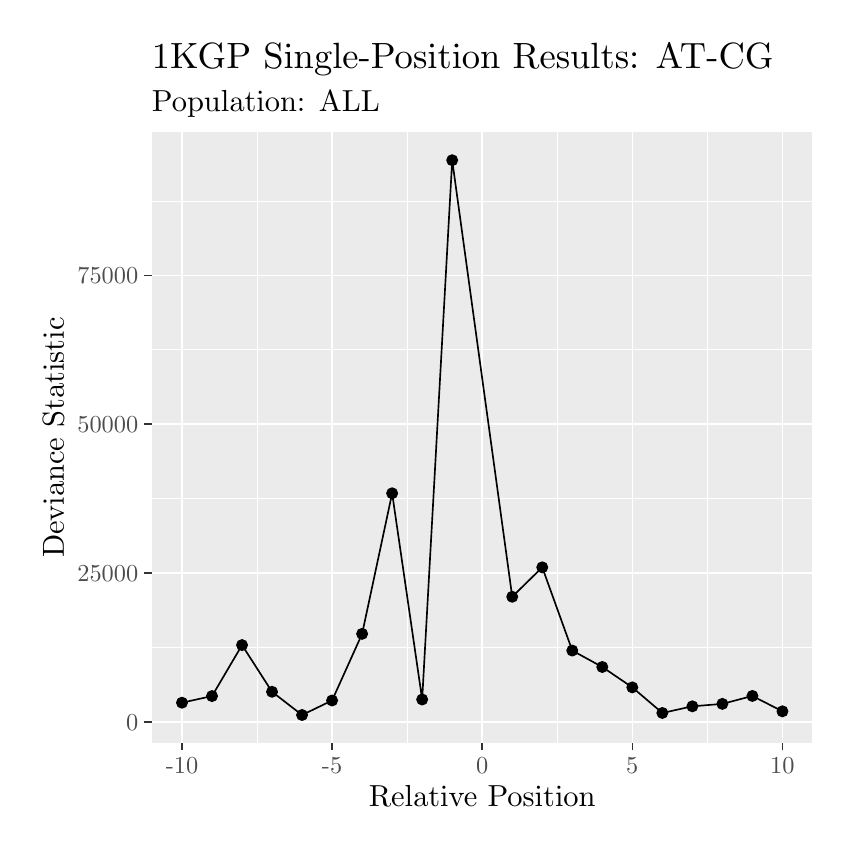
\begin{tikzpicture}[x=1pt,y=1pt]
\definecolor{fillColor}{RGB}{255,255,255}
\path[use as bounding box,fill=fillColor,fill opacity=0.00] (0,0) rectangle (289.08,289.08);
\begin{scope}
\path[clip] (  0.00,  0.00) rectangle (289.08,289.08);
\definecolor{drawColor}{RGB}{255,255,255}
\definecolor{fillColor}{RGB}{255,255,255}

\path[draw=drawColor,line width= 0.6pt,line join=round,line cap=round,fill=fillColor] (  0.00,  0.00) rectangle (289.08,289.08);
\end{scope}
\begin{scope}
\path[clip] ( 44.91, 30.69) rectangle (283.58,251.21);
\definecolor{fillColor}{gray}{0.92}

\path[fill=fillColor] ( 44.91, 30.69) rectangle (283.58,251.21);
\definecolor{drawColor}{RGB}{255,255,255}

\path[draw=drawColor,line width= 0.3pt,line join=round] ( 44.91, 65.10) --
	(283.58, 65.10);

\path[draw=drawColor,line width= 0.3pt,line join=round] ( 44.91,118.88) --
	(283.58,118.88);

\path[draw=drawColor,line width= 0.3pt,line join=round] ( 44.91,172.66) --
	(283.58,172.66);

\path[draw=drawColor,line width= 0.3pt,line join=round] ( 44.91,226.44) --
	(283.58,226.44);

\path[draw=drawColor,line width= 0.3pt,line join=round] ( 82.88, 30.69) --
	( 82.88,251.21);

\path[draw=drawColor,line width= 0.3pt,line join=round] (137.12, 30.69) --
	(137.12,251.21);

\path[draw=drawColor,line width= 0.3pt,line join=round] (191.37, 30.69) --
	(191.37,251.21);

\path[draw=drawColor,line width= 0.3pt,line join=round] (245.61, 30.69) --
	(245.61,251.21);

\path[draw=drawColor,line width= 0.6pt,line join=round] ( 44.91, 38.21) --
	(283.58, 38.21);

\path[draw=drawColor,line width= 0.6pt,line join=round] ( 44.91, 91.99) --
	(283.58, 91.99);

\path[draw=drawColor,line width= 0.6pt,line join=round] ( 44.91,145.77) --
	(283.58,145.77);

\path[draw=drawColor,line width= 0.6pt,line join=round] ( 44.91,199.55) --
	(283.58,199.55);

\path[draw=drawColor,line width= 0.6pt,line join=round] ( 55.76, 30.69) --
	( 55.76,251.21);

\path[draw=drawColor,line width= 0.6pt,line join=round] (110.00, 30.69) --
	(110.00,251.21);

\path[draw=drawColor,line width= 0.6pt,line join=round] (164.24, 30.69) --
	(164.24,251.21);

\path[draw=drawColor,line width= 0.6pt,line join=round] (218.49, 30.69) --
	(218.49,251.21);

\path[draw=drawColor,line width= 0.6pt,line join=round] (272.73, 30.69) --
	(272.73,251.21);
\definecolor{drawColor}{RGB}{0,0,0}
\definecolor{fillColor}{RGB}{0,0,0}

\path[draw=drawColor,line width= 0.4pt,line join=round,line cap=round,fill=fillColor] ( 55.76, 45.16) circle (  1.96);

\path[draw=drawColor,line width= 0.4pt,line join=round,line cap=round,fill=fillColor] ( 66.61, 47.55) circle (  1.96);

\path[draw=drawColor,line width= 0.4pt,line join=round,line cap=round,fill=fillColor] ( 77.46, 65.98) circle (  1.96);

\path[draw=drawColor,line width= 0.4pt,line join=round,line cap=round,fill=fillColor] ( 88.30, 49.10) circle (  1.96);

\path[draw=drawColor,line width= 0.4pt,line join=round,line cap=round,fill=fillColor] ( 99.15, 40.71) circle (  1.96);

\path[draw=drawColor,line width= 0.4pt,line join=round,line cap=round,fill=fillColor] (110.00, 45.96) circle (  1.96);

\path[draw=drawColor,line width= 0.4pt,line join=round,line cap=round,fill=fillColor] (120.85, 70.04) circle (  1.96);

\path[draw=drawColor,line width= 0.4pt,line join=round,line cap=round,fill=fillColor] (131.70,120.83) circle (  1.96);

\path[draw=drawColor,line width= 0.4pt,line join=round,line cap=round,fill=fillColor] (142.55, 46.32) circle (  1.96);

\path[draw=drawColor,line width= 0.4pt,line join=round,line cap=round,fill=fillColor] (153.40,241.18) circle (  1.96);

\path[draw=drawColor,line width= 0.4pt,line join=round,line cap=round,fill=fillColor] (175.09, 83.44) circle (  1.96);

\path[draw=drawColor,line width= 0.4pt,line join=round,line cap=round,fill=fillColor] (185.94, 94.07) circle (  1.96);

\path[draw=drawColor,line width= 0.4pt,line join=round,line cap=round,fill=fillColor] (196.79, 64.00) circle (  1.96);

\path[draw=drawColor,line width= 0.4pt,line join=round,line cap=round,fill=fillColor] (207.64, 58.06) circle (  1.96);

\path[draw=drawColor,line width= 0.4pt,line join=round,line cap=round,fill=fillColor] (218.49, 50.69) circle (  1.96);

\path[draw=drawColor,line width= 0.4pt,line join=round,line cap=round,fill=fillColor] (229.34, 41.45) circle (  1.96);

\path[draw=drawColor,line width= 0.4pt,line join=round,line cap=round,fill=fillColor] (240.19, 43.85) circle (  1.96);

\path[draw=drawColor,line width= 0.4pt,line join=round,line cap=round,fill=fillColor] (251.03, 44.73) circle (  1.96);

\path[draw=drawColor,line width= 0.4pt,line join=round,line cap=round,fill=fillColor] (261.88, 47.60) circle (  1.96);

\path[draw=drawColor,line width= 0.4pt,line join=round,line cap=round,fill=fillColor] (272.73, 42.04) circle (  1.96);

\path[draw=drawColor,line width= 0.6pt,line join=round] ( 55.76, 45.16) --
	( 66.61, 47.55) --
	( 77.46, 65.98) --
	( 88.30, 49.10) --
	( 99.15, 40.71) --
	(110.00, 45.96) --
	(120.85, 70.04) --
	(131.70,120.83) --
	(142.55, 46.32) --
	(153.40,241.18) --
	(175.09, 83.44) --
	(185.94, 94.07) --
	(196.79, 64.00) --
	(207.64, 58.06) --
	(218.49, 50.69) --
	(229.34, 41.45) --
	(240.19, 43.85) --
	(251.03, 44.73) --
	(261.88, 47.60) --
	(272.73, 42.04);
\end{scope}
\begin{scope}
\path[clip] (  0.00,  0.00) rectangle (289.08,289.08);
\definecolor{drawColor}{gray}{0.30}

\node[text=drawColor,anchor=base east,inner sep=0pt, outer sep=0pt, scale=  0.88] at ( 39.96, 35.18) {0};

\node[text=drawColor,anchor=base east,inner sep=0pt, outer sep=0pt, scale=  0.88] at ( 39.96, 88.96) {25000};

\node[text=drawColor,anchor=base east,inner sep=0pt, outer sep=0pt, scale=  0.88] at ( 39.96,142.74) {50000};

\node[text=drawColor,anchor=base east,inner sep=0pt, outer sep=0pt, scale=  0.88] at ( 39.96,196.52) {75000};
\end{scope}
\begin{scope}
\path[clip] (  0.00,  0.00) rectangle (289.08,289.08);
\definecolor{drawColor}{gray}{0.20}

\path[draw=drawColor,line width= 0.6pt,line join=round] ( 42.16, 38.21) --
	( 44.91, 38.21);

\path[draw=drawColor,line width= 0.6pt,line join=round] ( 42.16, 91.99) --
	( 44.91, 91.99);

\path[draw=drawColor,line width= 0.6pt,line join=round] ( 42.16,145.77) --
	( 44.91,145.77);

\path[draw=drawColor,line width= 0.6pt,line join=round] ( 42.16,199.55) --
	( 44.91,199.55);
\end{scope}
\begin{scope}
\path[clip] (  0.00,  0.00) rectangle (289.08,289.08);
\definecolor{drawColor}{gray}{0.20}

\path[draw=drawColor,line width= 0.6pt,line join=round] ( 55.76, 27.94) --
	( 55.76, 30.69);

\path[draw=drawColor,line width= 0.6pt,line join=round] (110.00, 27.94) --
	(110.00, 30.69);

\path[draw=drawColor,line width= 0.6pt,line join=round] (164.24, 27.94) --
	(164.24, 30.69);

\path[draw=drawColor,line width= 0.6pt,line join=round] (218.49, 27.94) --
	(218.49, 30.69);

\path[draw=drawColor,line width= 0.6pt,line join=round] (272.73, 27.94) --
	(272.73, 30.69);
\end{scope}
\begin{scope}
\path[clip] (  0.00,  0.00) rectangle (289.08,289.08);
\definecolor{drawColor}{gray}{0.30}

\node[text=drawColor,anchor=base,inner sep=0pt, outer sep=0pt, scale=  0.88] at ( 55.76, 19.68) {-10};

\node[text=drawColor,anchor=base,inner sep=0pt, outer sep=0pt, scale=  0.88] at (110.00, 19.68) {-5};

\node[text=drawColor,anchor=base,inner sep=0pt, outer sep=0pt, scale=  0.88] at (164.24, 19.68) {0};

\node[text=drawColor,anchor=base,inner sep=0pt, outer sep=0pt, scale=  0.88] at (218.49, 19.68) {5};

\node[text=drawColor,anchor=base,inner sep=0pt, outer sep=0pt, scale=  0.88] at (272.73, 19.68) {10};
\end{scope}
\begin{scope}
\path[clip] (  0.00,  0.00) rectangle (289.08,289.08);
\definecolor{drawColor}{RGB}{0,0,0}

\node[text=drawColor,anchor=base,inner sep=0pt, outer sep=0pt, scale=  1.10] at (164.24,  7.64) {Relative Position};
\end{scope}
\begin{scope}
\path[clip] (  0.00,  0.00) rectangle (289.08,289.08);
\definecolor{drawColor}{RGB}{0,0,0}

\node[text=drawColor,rotate= 90.00,anchor=base,inner sep=0pt, outer sep=0pt, scale=  1.10] at ( 13.08,140.95) {Deviance Statistic};
\end{scope}
\begin{scope}
\path[clip] (  0.00,  0.00) rectangle (289.08,289.08);
\definecolor{drawColor}{RGB}{0,0,0}

\node[text=drawColor,anchor=base west,inner sep=0pt, outer sep=0pt, scale=  1.10] at ( 44.91,258.85) {Population: ALL};
\end{scope}
\begin{scope}
\path[clip] (  0.00,  0.00) rectangle (289.08,289.08);
\definecolor{drawColor}{RGB}{0,0,0}

\node[text=drawColor,anchor=base west,inner sep=0pt, outer sep=0pt, scale=  1.32] at ( 44.91,274.49) {1KGP Single-Position Results: AT-CG};
\end{scope}
\end{tikzpicture}
